\chapter{Software Modules} % Main chapter title

\section*{4.1 \hspace{1cm} DB Normalization}
\subsection*{4.1.1 \hspace{1cm} ER}
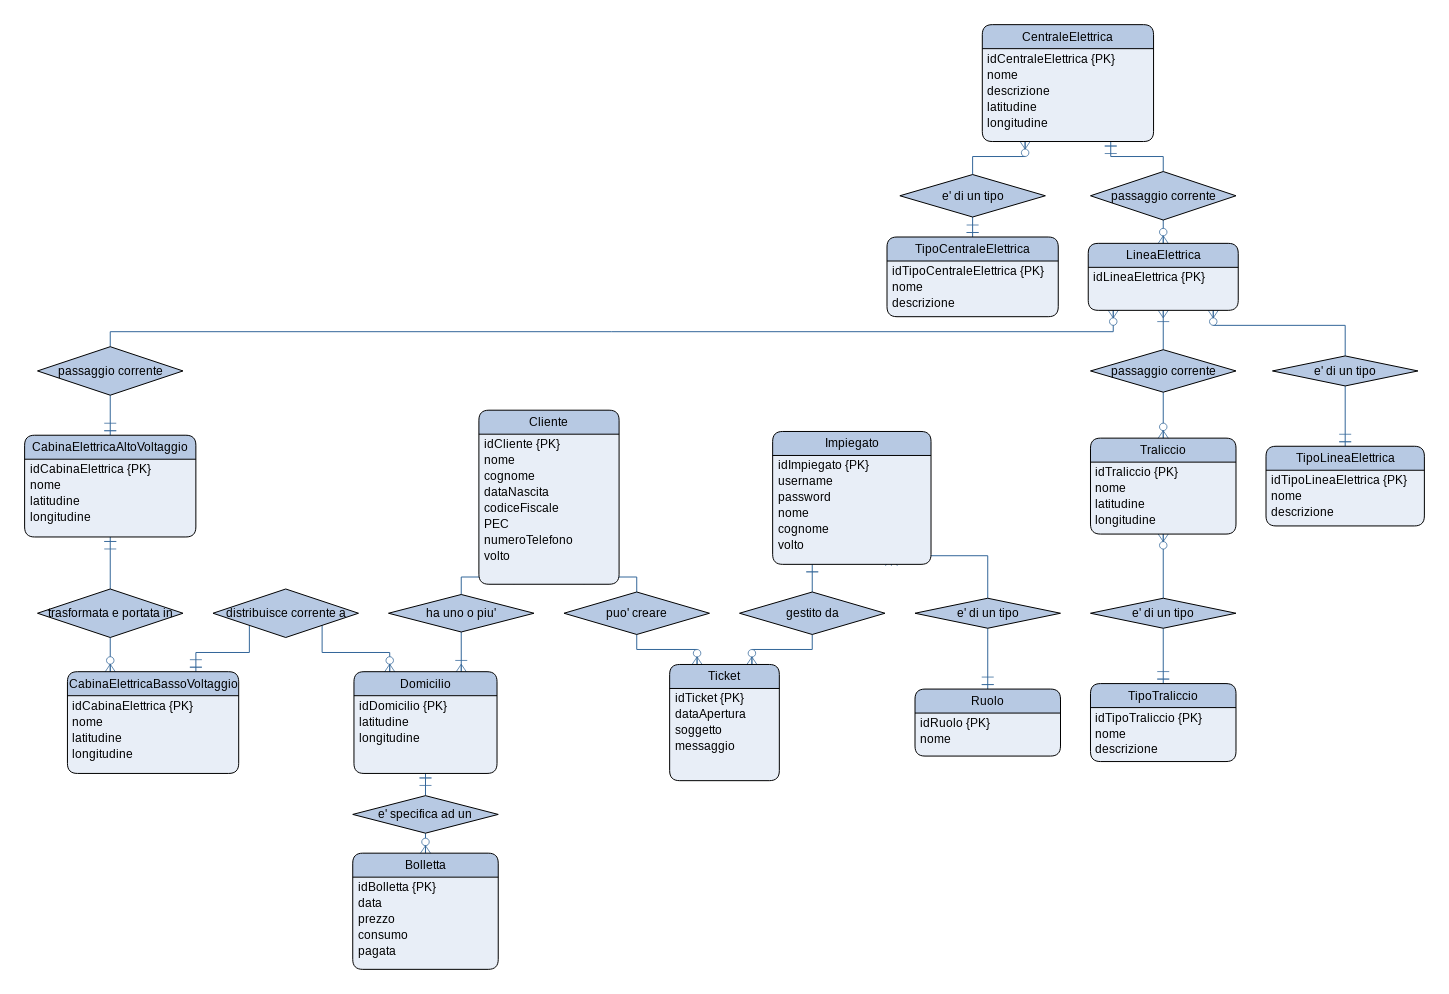
\includegraphics[width=\linewidth]{Figures/ER.png}
\subsection * {4.1.2 \hspace {1cm} 1FN}
The scheme is in 1st normal form since all its attributes are atomic and have the same type. \\
The first normalization form is the easiest, you just need to respect the basic rules, which are:
\begin {itemize}
    \item not using compount fields
    \item having the same number of rows and columns
    \item all records are unique
\end {itemize}

\subsection * {4.1.3 \hspace {1cm} 2FN}
Since we don't have compound keys, we don't need to do anything to check 2nd normal form. \\

\subsection * {4.1.3 \hspace {1cm} 3FN}
All columns directly depend on the primary key, it is reduced to 3rd normal form. \\

\section*{4.2 \hspace{1cm} Logic Scheme}

\begin{center}
    \begin{tabular}{ |l|c|c|c|c|c|c| } 
        \hline
        \multicolumn{7}{|c|}{CentraleElettrica} \\
        \hline
            Name        & Type      & Size  & Key       & Null  & Default   & Extra \\
        \hline
            idCentrale  & INTEGER   &       & PRIMARY   & NO    &           & AUTO INCREMENT \\
            nome        & VARCHAR   & 128   &           & NO    &           &                \\
            latitudine  & FLOAT     &       &           & NO    &           &                \\
            longitudine & FLOAT     &       &           & NO    &           &                \\
        \hline
    \end{tabular}
\end{center}


\begin{center}
    \begin{tabular}{ |l|c|c|c|c|c|c| } 
        \hline
        \multicolumn{7}{|c|}{LineaElettrica} \\
        \hline
            Name             & Type     & Size  & Key       & Null  & Default   & Extra \\
        \hline
            idLineaElettrica & INTEGER  &       & PRIMARY   & NO    &           & AUTO INCREMENT \\
            origine          & INTEGER  &       & FOREIGN   & NO    &           & \\
            destinazione     & INTEGER  &       & FOREIGN   & NO    &           & \\
        \hline
    \end{tabular}
\end{center}

\begin{center}
    \begin{tabular}{ |l|c|c|c|c|c|c| } 
        \hline
        \multicolumn{7}{|c|}{Cabina} \\
        \hline
            Name             & Type     & Size  & Key       & Null  & Default   & Extra \\
        \hline
            idCabina         & INTEGER  &       & PRIMARY   & NO    &           & AUTO INCREMENT \\
            nome             & VARCHAR  & 128   &           & YES   &           & \\
            latitudine       & FLOAT    &       &           & NO    &           & \\
            longitudine      & FLOAT    &       &           & NO    &           & \\
        \hline
    \end{tabular}
\end{center}

\begin{center}
    \begin{tabular}{ |l|c|c|c|c|c|c| } 
        \hline
        \multicolumn{7}{|c|}{PassaggioLinea} \\
        \hline
            Name                    & Type     & Size   & Key       & Null  & Default   & Extra \\
        \hline
            idPassaggio             & INTEGER  &        & PRIMARY   & NO    &           & AUTO INCREMENT \\
            idLinea                 & INTEGER  &        & FOREIGN   & NO    & 1         & \\
            iterazione              & INTEGER  &        &           & NO    &           & AUTO INCREMENT \\
            idTraliccioOrigine      & INTEGER  &        & FOREIGN   & NO    &           & \\
            idTraliccioDestinazione & INTEGER  &        & FOREIGN   & NO    &           & \\
        \hline
    \end{tabular}
\end{center}

\begin{center}
    \begin{tabular}{ |l|c|c|c|c|c|c| } 
        \hline
        \multicolumn{7}{|c|}{Traliccio} \\
        \hline
            Name             & Type     & Size  & Key       & Null  & Default   & Extra \\
        \hline
            idTraliccio      & INTEGER  &       & PRIMARY   & NO    &           & AUTO INCREMENT \\
            latitude         & FLOAT    &       &           & NO    &           & \\
            longitude        & FLOAT    &       &           & NO    &           & \\
        \hline
    \end{tabular}
\end{center}

\begin{center}
    \begin{tabular}{ |l|c|c|c|c|c|c| } 
        \hline
        \multicolumn{7}{|c|}{Cliente} \\
        \hline
            Name             & Type     & Size  & Key       & Null  & Default   & Extra \\
        \hline
            idCliente        & INTEGER  &       & PRIMARY   & NO    &           & AUTO INCREMENT \\
            nome             & VARCHAR  & 64    &           & NO    &           & \\
            cognome          & VARCHAR  & 64    &           & NO    &           & \\
            dataNascita      & DATE     &       &           & NO    &           & \\
            codiceFiscale    & VARCHAR  & 16    &           & NO    &           & UNIQUE \\
            numeroTelefono   & VARCHAR  & 16    &           & NO    &           & UNIQUE \\
            email            & VARCHAR  & 300   &           & NO    &           & UNIQUE \\
        \hline
    \end{tabular}
\end{center}
\begin{center}
    \begin{tabular}{ |l|c|c|c|c|c|c| } 
        \hline
        \multicolumn{7}{|c|}{Domicilio} \\
        \hline
            Name             & Type     & Size  & Key       & Null  & Default   & Extra \\
        \hline
            idDomicilio      & INTEGER  &       & PRIMARY   & NO    &           & AUTO INCREMENT \\
            idCliente        & INTEGER  &       & FOREIGN   & NO    &           & \\
            latitudine       & FLOAT    &       &           & NO    &           & \\
            longitudine      & FLOAT    &       &           & NO    &           & \\
            idLineaElettrica & INTEGER  &       & FOREIGN   & NO    &           & \\
        \hline
    \end{tabular}
\end{center}
\begin{center}
    \begin{tabular}{ |l|c|c|c|c|c|c| } 
        \hline
        \multicolumn{7}{|c|}{Bolletta} \\
        \hline
            Name             & Type     & Size  & Key       & Null  & Default   & Extra \\
        \hline
            idBolletta       & INTEGER  &       & PRIMARY   & NO    &           & AUTO INCREMENT \\
            idDomicilio      & INTEGER  &       & FOREIGN   & NO    &           & \\
            consumoWatt      & FLOAT    &       &           & NO    & 0         & \\
            dataBolletta     & DATE     &       &           & NO    & CURDATE   & \\
            pagata           & BOOLEAN  &       &           & NO    & FALSE     & \\
        \hline
    \end{tabular}
\end{center}
\begin{center}
    \begin{tabular}{ |l|c|c|c|c|c|c| } 
        \hline
        \multicolumn{7}{|c|}{Impiegato} \\
        \hline
            Name             & Type     & Size  & Key       & Null  & Default   & Extra \\
        \hline
            idImpiegato      & INTEGER  &       & PRIMARY   & NO    &           & AUTO INCREMENT \\
            username         & VARCHAR  & 300   &           & NO    &           & UNIQUE \\
            password         & CHAR     & 128   &           & NO    &           & \\
            nome             & VARCHAR  & 64    &           & NO    &           & \\
            cognome          & VARCHAR  & 64    &           & NO    &           & \\
            ruolo            & INTEGER  &       & FOREIGN   & NO    &           & \\
        \hline
    \end{tabular}
\end{center}

\section*{4.3 \hspace{1cm} DDL}
\subsection*{Traditional Method}
The traditional method is not used in this project.
\lstinputlisting[language=SQL]{Code/ddl.sql}

\subsection*{The SQLAlchemy Way}
\begin{verbatim*}
restricted/code/models.py
\end{verbatim*}

\lstinputlisting[language=Python]{../../../project/api/code/models.py}


Per creare le tabelle del database:
\begin{lstlisting}[language=Python]
# Da qualsiasi parte
db = SQLAlchemy(app)
db.create_db()
\end{lstlisting}


\section*{4.4 \hspace{1cm} Inserting data}
\subsection*{Traditional method}
\lstinputlisting[language=SQL]{Code/data.sql}

\subsection*{The SQLAlchemy Way}
\lstinputlisting[language=Python]{../../../project/api/code/data/users.py}


\section*{4.5 \hspace{1cm} Some queries}
\subsection*{4.5.1 \hspace{1cm} Members of the financing team}
\subsubsection*{Traditional Method}
\lstinputlisting[language=SQL]{Code/query-1.sql}

\subsubsection*{The SQLAlchemy Way}
\begin{lstlisting}[language=Python]
User.query.filter_by(role=Role.query.filter_by(name='Finances')[0].id)
\end{lstlisting}


\section*{4.5.2 \hspace{1cm} Green Power Plants}
\subsection*{Traditional Method}
\lstinputlisting[language=SQL]{Code/query-2.sql}

\subsubsection*{The SQLAlchemy Way}
\begin{lstlisting}[language=Python]
    PowerPlant.query.filter(
        PowerPlant.category.in_(
            PowerPlantCategory.query.filter_by(name='Hydro')[0].id,
            PowerPlantCategory.query.filter_by(name='Solar')[0].id,
            PowerPlantCategory.query.filter_by(name='Wind')[0].id,
            PowerPlantCategory.query.filter_by(name='Nuclear')[0].id,
            PowerPlantCategory.query.filter_by(name='Geothermal')[0].id,
        )
    )
\end{lstlisting}
